\documentclass{standalone}
\usepackage{tikz}
\usetikzlibrary{patterns, positioning}
\usepackage[sfdefault]{ClearSans} %% option 'sfdefault' activates Clear Sans as the default text font
\usepackage[T1]{fontenc}

\begin{document}
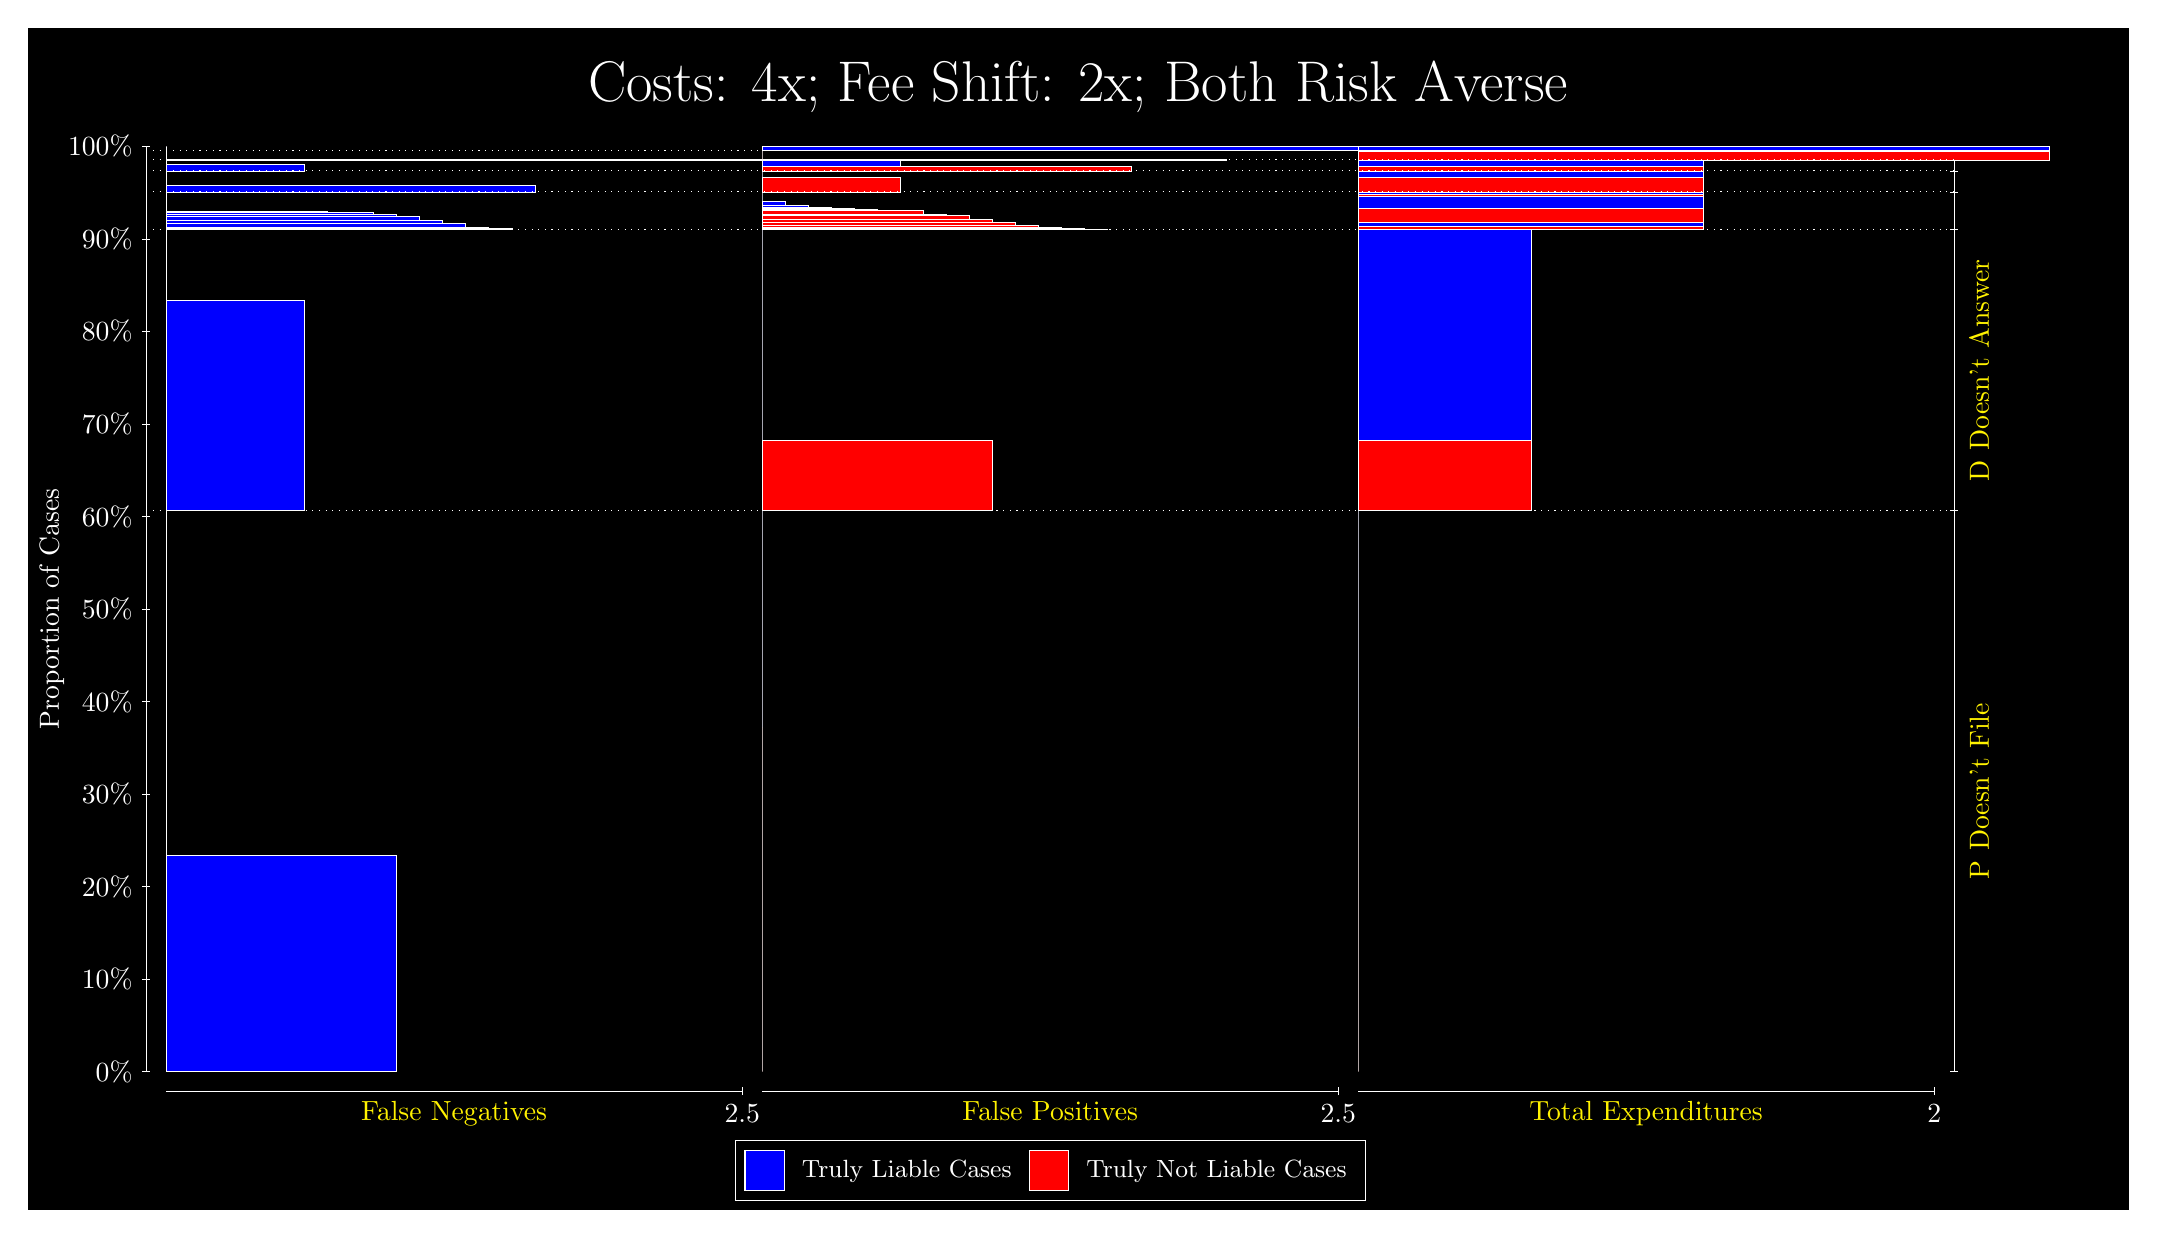
\begin{tikzpicture}
\draw[fill=black] (0,0) rectangle (26.667,15);
\draw[text=white] (0,13.5) rectangle (26.667,15) node[midway] {\huge Costs: 4x; Fee Shift: 2x; Both Risk Averse};
\draw[white, very thin] (1.5,1.75) -- (1.5,13.5);
\node[rotate=90, text=white, anchor=center] at (0.3, 7.625) {Proportion of Cases};
\draw[white, very thin] (1.45,1.75) -- (1.55,1.75);
\node[text=white, anchor=east] at (1.45, 1.75) {0\%};
\draw[white, very thin] (1.45,2.925) -- (1.55,2.925);
\node[text=white, anchor=east] at (1.45, 2.925) {10\%};
\draw[white, very thin] (1.45,4.1) -- (1.55,4.1);
\node[text=white, anchor=east] at (1.45, 4.1) {20\%};
\draw[white, very thin] (1.45,5.275) -- (1.55,5.275);
\node[text=white, anchor=east] at (1.45, 5.275) {30\%};
\draw[white, very thin] (1.45,6.45) -- (1.55,6.45);
\node[text=white, anchor=east] at (1.45, 6.45) {40\%};
\draw[white, very thin] (1.45,7.625) -- (1.55,7.625);
\node[text=white, anchor=east] at (1.45, 7.625) {50\%};
\draw[white, very thin] (1.45,8.8) -- (1.55,8.8);
\node[text=white, anchor=east] at (1.45, 8.8) {60\%};
\draw[white, very thin] (1.45,9.975) -- (1.55,9.975);
\node[text=white, anchor=east] at (1.45, 9.975) {70\%};
\draw[white, very thin] (1.45,11.15) -- (1.55,11.15);
\node[text=white, anchor=east] at (1.45, 11.15) {80\%};
\draw[white, very thin] (1.45,12.325) -- (1.55,12.325);
\node[text=white, anchor=east] at (1.45, 12.325) {90\%};
\draw[white, very thin] (1.45,13.5) -- (1.55,13.5);
\node[text=white, anchor=east] at (1.45, 13.5) {100\%};

\draw[white, very thin] (24.457,1.75) -- (24.457,13.5);
\draw[white, very thin] (24.407,1.75) -- (24.507,1.75);
\node[anchor=west] at (24.407, 1.75) {};
\draw[white, very thin] (24.407,8.8719) -- (24.507,8.8719);
\node[anchor=west] at (24.407, 8.8719) {};
\draw[white, very thin] (24.407,12.443) -- (24.507,12.443);
\node[anchor=west] at (24.407, 12.443) {};
\draw[white, very thin] (24.407,12.921) -- (24.507,12.921);
\node[anchor=west] at (24.407, 12.921) {};
\draw[white, very thin] (24.407,13.188) -- (24.507,13.188);
\node[anchor=west] at (24.407, 13.188) {};
\draw[white, very thin] (24.407,13.328) -- (24.507,13.328);
\node[anchor=west] at (24.407, 13.328) {};
\draw[white, very thin] (24.407,13.449) -- (24.507,13.449);
\node[anchor=west] at (24.407, 13.449) {};
\draw[white, very thin] (24.407,13.5) -- (24.507,13.5);
\node[anchor=west] at (24.407, 13.5) {};

\draw[white, very thin, fill=blue] (1.75,1.75) rectangle (4.6775,4.4981);
\draw[white, very thin, fill=red] (1.75,4.4981) rectangle (1.75,8.8719);
\draw[white, very thin, fill=blue] (1.75,8.8719) rectangle (3.5065,11.547);
\draw[white, very thin, fill=red] (1.75,11.547) rectangle (1.75,12.443);
\draw[white, very thin, fill=blue] (1.75,12.443) rectangle (6.1413,12.458);
\draw[white, very thin, fill=blue] (1.75,12.458) rectangle (5.8486,12.472);
\draw[white, very thin, fill=blue] (1.75,12.472) rectangle (5.5558,12.518);
\draw[white, very thin, fill=blue] (1.75,12.518) rectangle (5.2631,12.558);
\draw[white, very thin, fill=blue] (1.75,12.558) rectangle (4.9703,12.608);
\draw[white, very thin, fill=blue] (1.75,12.608) rectangle (4.6775,12.634);
\draw[white, very thin, fill=blue] (1.75,12.634) rectangle (4.3848,12.657);
\draw[white, very thin, fill=blue] (1.75,12.657) rectangle (4.092,12.668);
\draw[white, very thin, fill=blue] (1.75,12.668) rectangle (3.7993,12.674);
\draw[white, very thin, fill=red] (1.75,12.674) rectangle (1.75,12.921);
\draw[white, very thin, fill=blue] (1.75,12.921) rectangle (6.4341,13.003);
\draw[white, very thin, fill=red] (1.75,13.003) rectangle (1.75,13.188);
\draw[white, very thin, fill=blue] (1.75,13.188) rectangle (3.5065,13.271);
\draw[white, very thin, fill=red] (1.75,13.271) rectangle (1.75,13.328);
\draw[white, very thin, fill=blue] (1.75,13.328) rectangle (15.217,13.338);
\draw[white, very thin, fill=red] (1.75,13.338) rectangle (1.75,13.449);
\draw[white, very thin, fill=red] (1.75,13.449) rectangle (1.75,13.455);
\draw[white, very thin, fill=blue] (1.75,13.455) rectangle (1.75,13.5);
\draw[white, very thin, fill=red] (9.3189,1.75) rectangle (9.3189,6.1238);
\draw[white, very thin, fill=blue] (9.3189,6.1238) rectangle (9.3189,8.8719);
\draw[white, very thin, fill=red] (9.3189,8.8719) rectangle (12.246,9.7673);
\draw[white, very thin, fill=blue] (9.3189,9.7673) rectangle (9.3189,12.443);
\draw[white, very thin, fill=red] (9.3189,12.443) rectangle (13.71,12.449);
\draw[white, very thin, fill=red] (9.3189,12.449) rectangle (13.417,12.456);
\draw[white, very thin, fill=red] (9.3189,12.456) rectangle (13.125,12.474);
\draw[white, very thin, fill=red] (9.3189,12.474) rectangle (12.832,12.499);
\draw[white, very thin, fill=red] (9.3189,12.499) rectangle (12.539,12.54);
\draw[white, very thin, fill=red] (9.3189,12.54) rectangle (12.246,12.573);
\draw[white, very thin, fill=red] (9.3189,12.573) rectangle (11.954,12.618);
\draw[white, very thin, fill=red] (9.3189,12.618) rectangle (11.661,12.635);
\draw[white, very thin, fill=red] (9.3189,12.635) rectangle (11.368,12.69);
\draw[white, very thin, fill=blue] (9.3189,12.69) rectangle (10.783,12.696);
\draw[white, very thin, fill=blue] (9.3189,12.696) rectangle (10.49,12.707);
\draw[white, very thin, fill=blue] (9.3189,12.707) rectangle (10.197,12.73);
\draw[white, very thin, fill=blue] (9.3189,12.73) rectangle (9.9044,12.756);
\draw[white, very thin, fill=blue] (9.3189,12.756) rectangle (9.6116,12.805);
\draw[white, very thin, fill=blue] (9.3189,12.805) rectangle (9.3189,12.921);
\draw[white, very thin, fill=red] (9.3189,12.921) rectangle (11.075,13.106);
\draw[white, very thin, fill=blue] (9.3189,13.106) rectangle (9.3189,13.188);
\draw[white, very thin, fill=red] (9.3189,13.188) rectangle (14.003,13.245);
\draw[white, very thin, fill=blue] (9.3189,13.245) rectangle (11.075,13.328);
\draw[white, very thin, fill=red] (9.3189,13.328) rectangle (9.3189,13.439);
\draw[white, very thin, fill=blue] (9.3189,13.439) rectangle (9.3189,13.449);
\draw[white, very thin, fill=red] (9.3189,13.449) rectangle (22.786,13.455);
\draw[white, very thin, fill=blue] (9.3189,13.455) rectangle (19.858,13.5);
\draw[white, very thin, fill=red] (16.888,1.75) rectangle (16.888,6.1238);
\draw[white, very thin, fill=blue] (16.888,6.1238) rectangle (16.888,8.8719);
\draw[white, very thin, fill=red] (16.888,8.8719) rectangle (19.083,9.7673);
\draw[white, very thin, fill=blue] (16.888,9.7673) rectangle (19.083,12.443);
\draw[white, very thin, fill=red] (16.888,12.443) rectangle (21.279,12.484);
\draw[white, very thin, fill=blue] (16.888,12.484) rectangle (21.279,12.534);
\draw[white, very thin, fill=red] (16.888,12.534) rectangle (21.279,12.714);
\draw[white, very thin, fill=blue] (16.888,12.714) rectangle (21.279,12.862);
\draw[white, very thin, fill=red] (16.888,12.862) rectangle (21.279,12.887);
\draw[white, very thin, fill=blue] (16.888,12.887) rectangle (21.279,12.921);
\draw[white, very thin, fill=red] (16.888,12.921) rectangle (21.279,13.106);
\draw[white, very thin, fill=blue] (16.888,13.106) rectangle (21.279,13.188);
\draw[white, very thin, fill=red] (16.888,13.188) rectangle (21.279,13.245);
\draw[white, very thin, fill=blue] (16.888,13.245) rectangle (21.279,13.328);
\draw[white, very thin, fill=red] (16.888,13.328) rectangle (25.67,13.439);
\draw[white, very thin, fill=blue] (16.888,13.439) rectangle (25.67,13.449);
\draw[white, very thin, fill=red] (16.888,13.449) rectangle (25.67,13.455);
\draw[white, very thin, fill=blue] (16.888,13.455) rectangle (25.67,13.5);
\draw[white, dotted] (1.5,8.8719) -- (24.457,8.8719);
\draw[white, dotted] (1.5,12.443) -- (24.457,12.443);
\draw[white, dotted] (1.5,12.921) -- (24.457,12.921);
\draw[white, dotted] (1.5,13.188) -- (24.457,13.188);
\draw[white, dotted] (1.5,13.328) -- (24.457,13.328);
\draw[white, dotted] (1.5,13.449) -- (24.457,13.449);
\draw[white, very thin] (1.75,1.5) -- (9.0689,1.5);
\node[text=yellow, anchor=north] at (5.4094, 1.5) {False Negatives};
\draw[white, very thin] (9.0689,1.45) -- (9.0689,1.55);
\node[text=white, anchor=north] at (9.0689, 1.45) {2.5};

\draw[white, very thin] (9.3189,1.5) -- (16.638,1.5);
\node[text=yellow, anchor=north] at (12.978, 1.5) {False Positives};
\draw[white, very thin] (16.638,1.45) -- (16.638,1.55);
\node[text=white, anchor=north] at (16.638, 1.45) {2.5};

\draw[white, very thin] (16.888,1.5) -- (24.207,1.5);
\node[text=yellow, anchor=north] at (20.547, 1.5) {Total Expenditures};
\draw[white, very thin] (24.207,1.45) -- (24.207,1.55);
\node[text=white, anchor=north] at (24.207, 1.45) {2};

\node[text=yellow, centered, rotate=90] at (24.777, 5.311) {P Doesn't File};
\node[text=yellow, centered, rotate=90] at (24.777, 10.657) {D Doesn't Answer};






\draw (12.978300999999998,1.5) node[draw=none] (baseCoordinate) {};
\begin{scope}[align=center]
        \matrix[scale=0.5, draw=white, below=0.5cm of baseCoordinate, nodes={draw}, column sep=0.1cm]{
            \node[rectangle, draw, minimum width=0.5cm, minimum height=0.5cm, fill=blue] {}; &
            \node[draw=none, font=\small, text=white] (B) {Truly Liable Cases}; &
            \node[rectangle, draw, minimum width=0.5cm, minimum height=0.5cm, fill=red] {}; &
            \node[draw=none, font=\small, text=white] (B) {Truly Not Liable Cases}; \\
            };
\end{scope}

\end{tikzpicture}
\end{document}